\begin{enumerate}[leftmargin=2cm,labelsep=.5cm,label=\bfseries\alph*)]
	\item Draw a symbol for an SPDT switch: \\[5mm]
	\begin{circuitikz}[scale=2, transform shape] \draw
		(1,0) node[spdt] (myspdt) {}
		(0,0) -- (myspdt.in) 
		(myspdt.out 1) -- +(1,0)
		(myspdt.out 2) -- +(1,0);
	\end{circuitikz}
	\\[1cm]
	
	\item Draw a symbol for a 3P4T switch: \\
	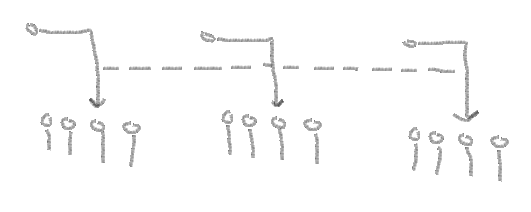
\includegraphics[scale=1]{gfx/3p4t.png}
	
	\item Decode the following resistor codes:
	\begin{enumerate}[label=\slshape\arabic*\normalfont)]
	\NumTabs{7}
		\item ORANGE-BLACK-BROWN-GOLD \tab{= \hlbox{$300\qw{\ohm}, \pm 5\%$}}
		\item BROWN-BLACK-YELLOW-GOLD \tab{= \hlbox{$100\qw{\kilo\ohm}, \pm 5\%$}}
		\item BLUE-GREY-BLACK-GOLD \tab{= \hlbox{$68\qw{\ohm}, \pm 5\%$}}
		\item RED-VIOLET-GREEN-GOLD \tab{= \hlbox{$2.7\qw{\mega\ohm}, \pm 5\%$}}
	\end{enumerate}
\end{enumerate}